\documentclass[twoside,10pt]{article}
\usepackage{amsmath,amsfonts,amsthm,fullpage}
\usepackage{algorithm}
\usepackage{algorithmic}
\usepackage{graphicx}
\usepackage{tcolorbox}


\begin{document}

\title{ISYE 6740 Fall 2020\\ Report}
%\author{Shasha Liao}
\date{}

\maketitle
\section{Image compression using clustering}

\subsection{k-medoids}
\begin{enumerate}
    \item In my k-medoids algorithm, I randomly generated $k$ pixels as the inital medoids for k clusters. (I also tried to randomly take $k$ pixels from the original picture, in which case the resulting number of clusters is very close to $k$.) My algorithm is designed to support three different kinds of similarity functions, including $l^1$, $l^2$ and $l^{\infty}$ norms. To update the representative of a cluster, I randomly choose a subset of $n\times 5\% + 1$ pixels from each cluster where $n$ is the total number of pixels in that cluster. Then for each pixel in the subset together with the old medoid, we assume it to be the new representative and calculate the objective function value inside the cluster. We choose the pixel with the least objective function value as the new representative for that cluster. My algorithm will terminate when two consecutive differences of objective function values are less than $10^{-8}$ or after 20 times of iterations. 
    
    \item I tried $k = 3,5,10,16,32$, and recorded the running times in seconds and number of iterations for convergence. My results are obtained using $l^1$ norm as the similarity function. I used my own flower picture (can be find below in part 3) to test the algorithm and plotted the results I obtained. The plot on the left shows that k-medoids is very slow to converge for the more complicated football picture, but faster for the simpler beach and flower pictures. Since for simpler pictures, there are a lot of pixels with the same values, so the difference matrix will end up with a lot of zeros, making it much easier to calculate similarities, label pixels and update medoids. Also, the first plot shows that as $k$ increases, the running time increases correspondingly. This is more obvious for complicated pictures like football. However, the plot on the right shows that the number of iterations seems like has no dependence on $k$. 
    
    \begin{center}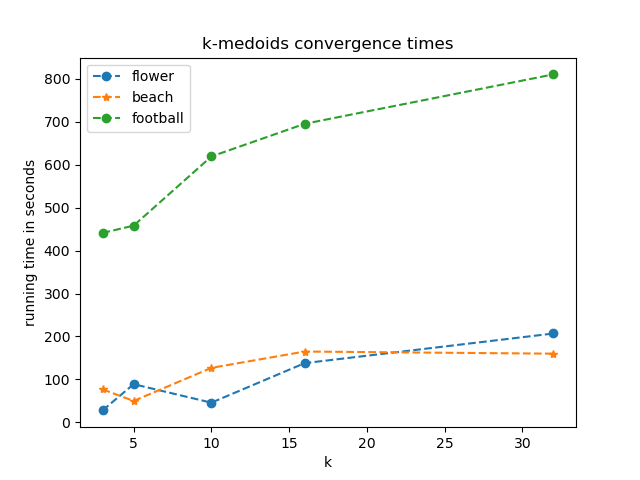
\includegraphics[scale=0.5]{kmedoids_times.png}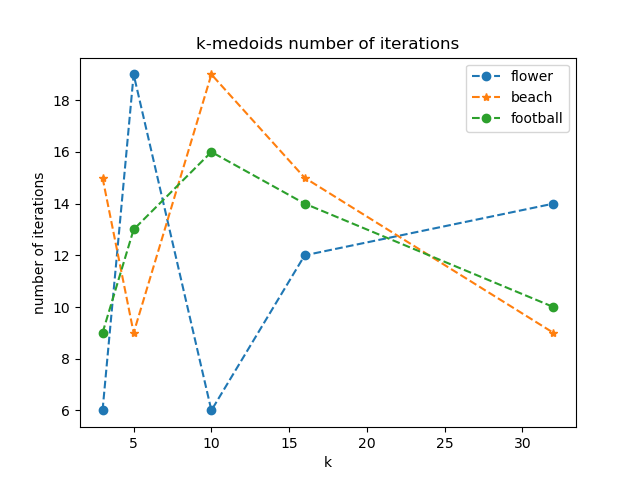
\includegraphics[scale=0.5]{kmedoids_iters.png}\end{center}
	
    
    
    \item The initial representations dose have affect in final results. Different initial representations result in different final resulting clusters. As we can see from the following pictures. The one on the top is the original picture. And the two pictures on the bottom were obtained by running kmedoids twice both with $k=8$, but different random initial representations.  
        \begin{center}
        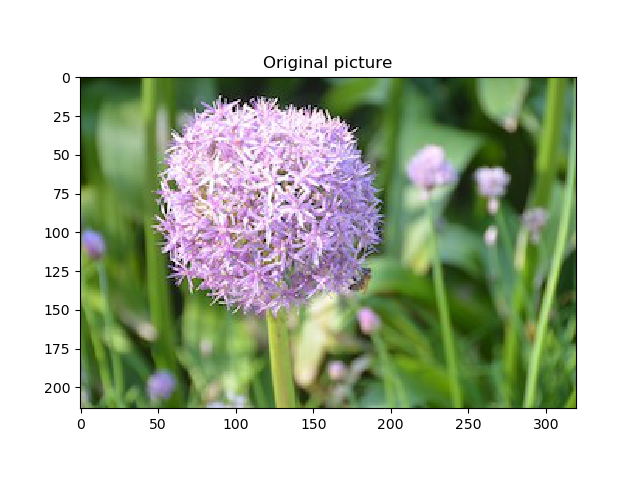
\includegraphics[scale = 0.5]{homework1/flower.png}
    \end{center}
     \begin{center}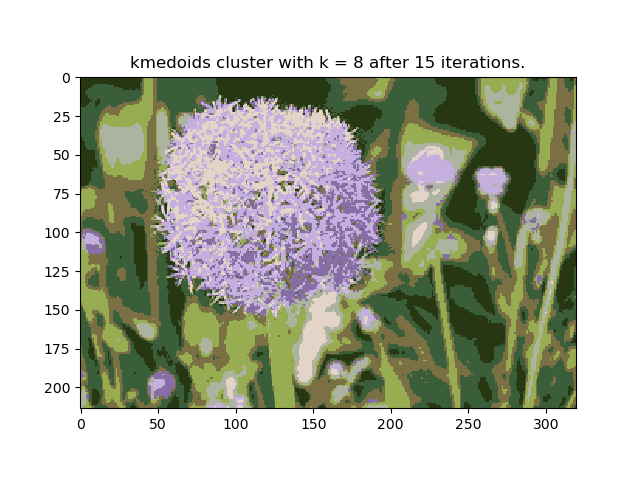
\includegraphics[scale=0.5]{kmedoids1.png}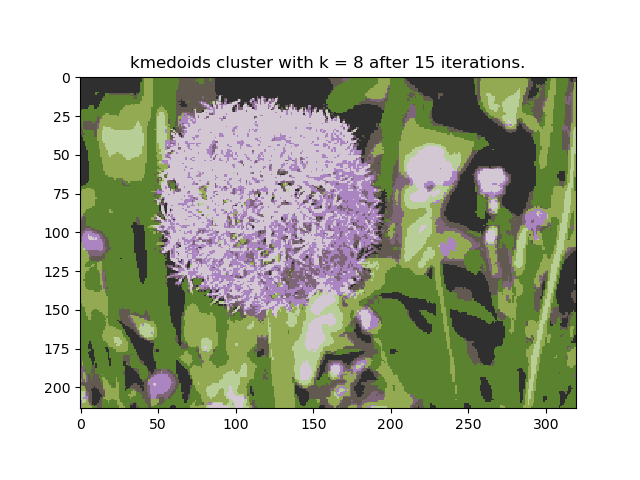
\includegraphics[scale=0.5]{kmedoids2.png}\end{center}
    
    \item Question 2 and 3 for kmeans are answered in the next subsection. In terms of the output quality, k-medoids did a better job because it uses the pixels from the original picture so that the color of the resulting compressed picture is much closer to the original picture. This is not the case for kmeans because the representative color for each cluster is obtained by averaging the colors in that cluster. Also, since k-medoids uses representative pixels from the original picture, it is more robust to noise and outliers compared to kmeans. 
    \begin{center}
        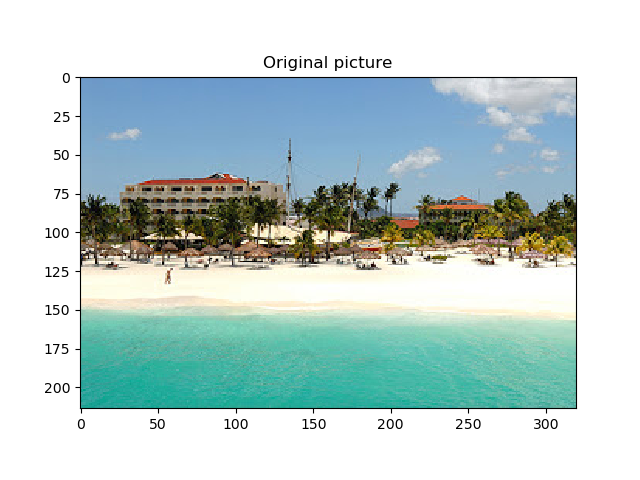
\includegraphics[scale = 0.5]{homework1/beach.png}
        \end{center}
    \begin{center}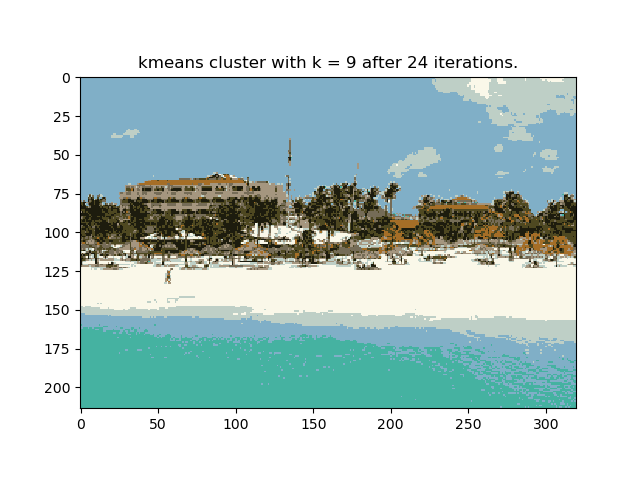
\includegraphics[scale=0.5]{beach_kmeans.png}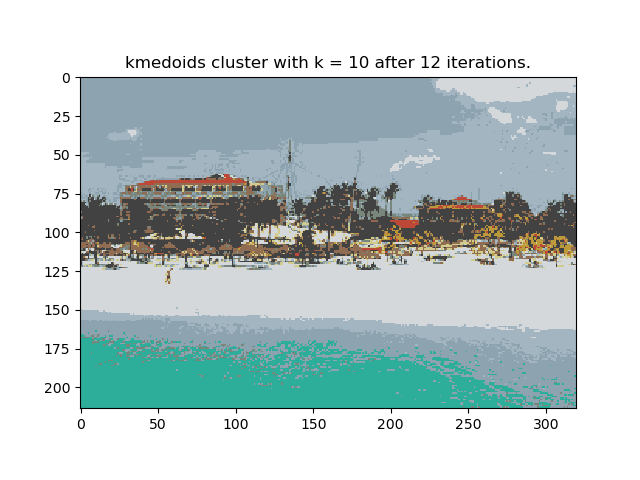
\includegraphics[scale=0.5]{beach_kmedoids.png}\end{center}
    
    However, kmeans has its own strength on efficiency since calculating the similarities and centroids are much easier compared with kmedoids as everything in kmeans can be done with matrix multiplications. The following plot compares the running time of kmeans and kmedoids on the picture of beach.
    \begin{center}
        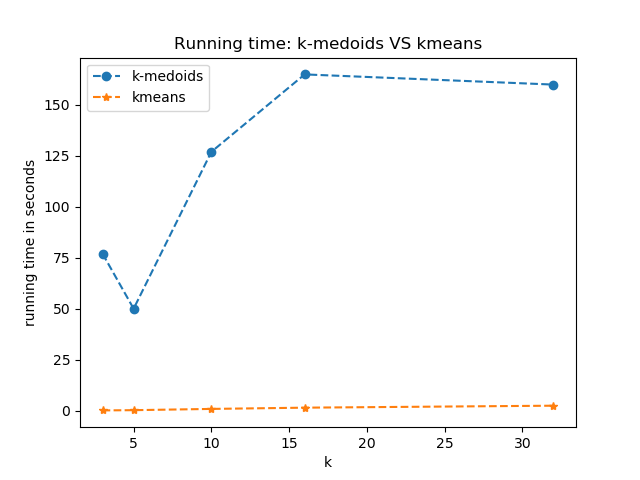
\includegraphics[scale=.5]{run_time_compare.png}
    \end{center}
    
    Besides, I have also observed the phenomenon that when $k$ is large, both the kmeans and kmedoids will result in less clusters. For example, when $k = 32$, both of the two clustering algorithms ended up with around 24 clusters, instead of 32 clusters. I believe this is related to the way the initial centroids/medoids were selected. As it shows, if we initialize medoids from the picture, than the resulting number of clusters will still be $k$ or at least very close to $k$.

\end{enumerate}


\subsection{kmeans}
\begin{enumerate}
    \item Nothing need to do for kmeans.
    \item I tried $k = 3,5,10,16,32$, and recorded the running times in seconds, number of iterations for convergence. The results can be easily seen from the following plots. As we can see, with $k$ increases, both the running times and the number of iterations increase. And when $k$ is large, the number of resulting clusters is much smaller than $k$. 

    \begin{center}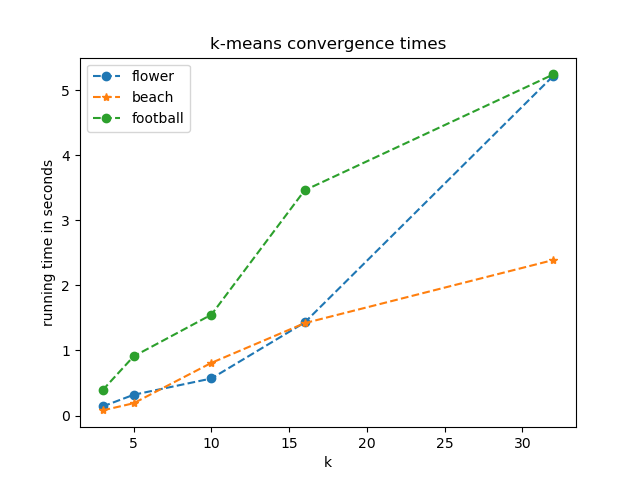
\includegraphics[scale=0.5]{kmeans_times.png}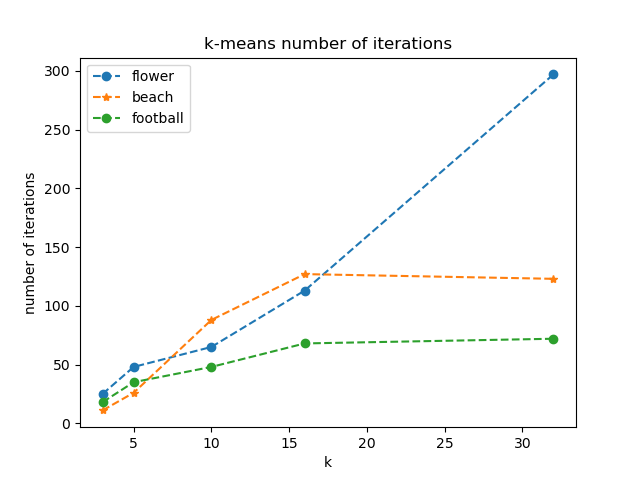
\includegraphics[scale=0.5]{kmeans_iters.png}\end{center}
    \item Different initial centroids will result in different resulting clusters. For example, I ran my kmeans with $k = 10$ and obtained the following different results. The picture on the left ended up with $k=10$. However, the picture on the right ended up with $k=7$. 
        \begin{center}
        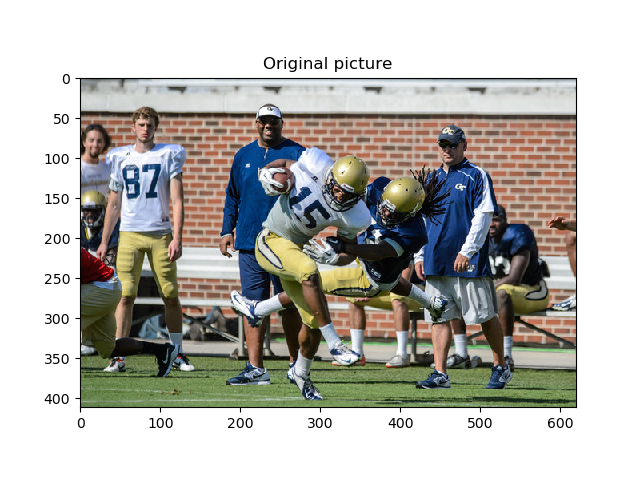
\includegraphics[scale = 0.5]{homework1/football.png}
        \end{center}
    \begin{center}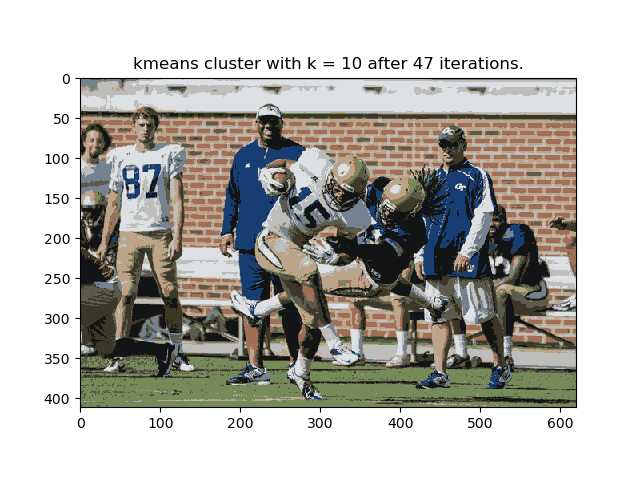
\includegraphics[scale=0.5]{kmeans1.png}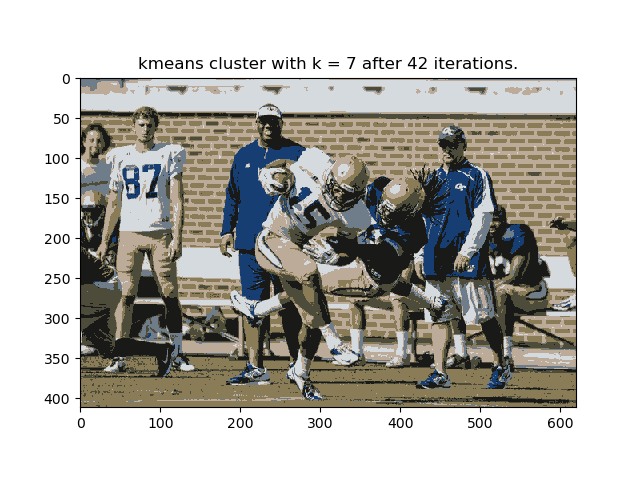
\includegraphics[scale=0.5]{homework1/kmeans2.png}\end{center}
\end{enumerate}

\end{document}